\documentclass[border=6pt]{standalone}
\usepackage[T1]{fontenc}
\usepackage{lmodern}\usepackage{tgtermes}
\usepackage{amsmath,amssymb,xcolor,tikz}
\usetikzlibrary{arrows.meta,calc,positioning}
\tikzset{
  bus/.style={line width=2.4pt},
  ln/.style={line width=0.8pt},
  gen/.style={circle, draw, line width=0.8pt, minimum size=9mm, inner sep=0pt, font=\small},
  load/.style={-{Stealth[length=2.6mm]}, line width=0.8pt},
  lab/.style={font=\footnotesize, fill=white, inner sep=1.5pt},
  res/.style={font=\footnotesize\bfseries, inner sep=1pt},
}


\begin{document}
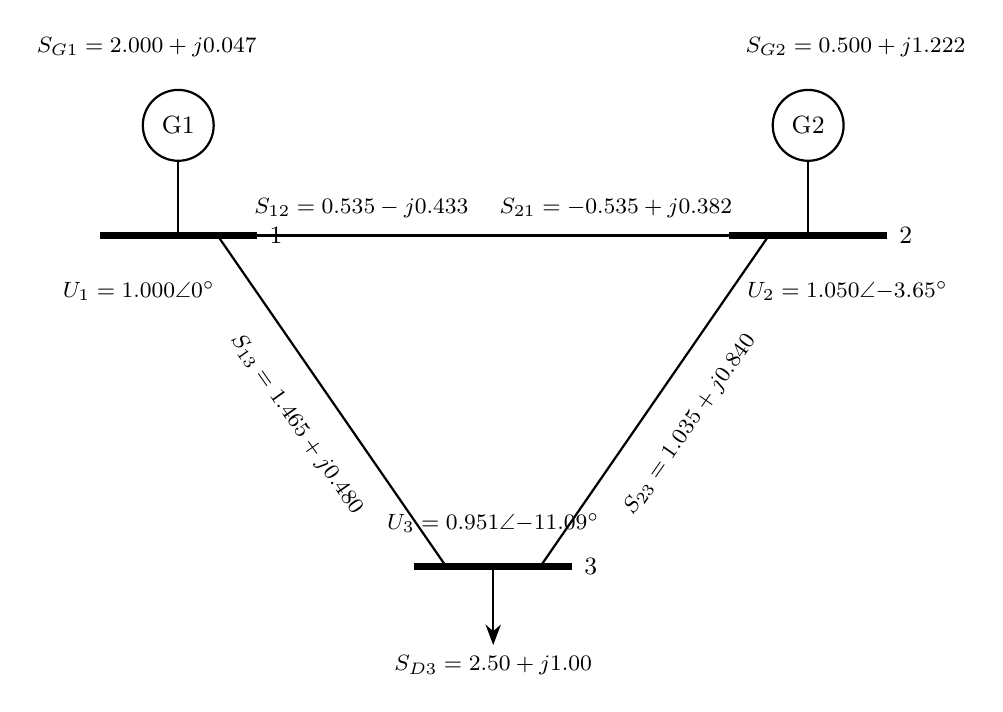
\begin{tikzpicture}[scale=1.0]
  \draw[bus] (-1.0,0) -- (1.0,0) node[right, font=\small] {1};
  \draw[bus] (7.0,0) -- (9.0,0) node[right, font=\small] {2};
  \draw[bus] (3.0,-4.2) -- (5.0,-4.2) node[right, font=\small] {3};
  \node[gen] (g1) at (0,1.4) {G1}; \draw[ln] (g1) -- (0,0);
  \node[gen] (g2) at (8,1.4) {G2}; \draw[ln] (g2) -- (8,0);
  \draw[load] (4,-4.2) -- (4,-5.2) node[below, font=\footnotesize] {$S_{D3} = 2.50 + j1.00$};
  \draw[ln] (0.8,0) -- (7.2,0) ; \draw[ln] (0.5,0) -- (3.4,-4.2); \draw[ln] (7.5,0) -- (4.6,-4.2);
  \node[lab] at (4,0.35) {$S_{12} = 0.535 - j0.433$ \quad $S_{21} = -0.535 + j0.382$};
  \node[lab, rotate=-55] at (1.5,-2.4) {$S_{13} = 1.465 + j0.480$};
  \node[lab, rotate=55] at (6.5,-2.4) {$S_{23} = 1.035 + j0.840$};
  \node[res, align=left] at (-0.5,-0.7) {$U_1 = 1.000\angle 0^\circ$};
  \node[res, align=left] at (8.5,-0.7) {$U_2 = 1.050\angle{-3.65}^\circ$};
  \node[res] at (4,-3.65) {$U_3 = 0.951\angle{-11.09}^\circ$};
  \node[font=\footnotesize, align=left] at (-0.4,2.4) {$S_{G1} = 2.000 + j0.047$};
  \node[font=\footnotesize, align=left] at (8.6,2.4) {$S_{G2} = 0.500 + j1.222$};
\end{tikzpicture}
\end{document}
